\newcommand{\svcourse}{CST Part IA: Software Engineering and Security}
\newcommand{\svnumber}{1}
\newcommand{\svvenue}{Microsoft Teams}
\newcommand{\svdate}{2022-05-11}
\newcommand{\svtime}{15:00}
\newcommand{\svuploadkey}{CBd13xmL7PC1zqhNIoLdTiYUBnxZhzRAtJxv/ytRdM1r7qIfwMsxeVwM/pPcIo8l}

\newcommand{\svrname}{Dr Sam Ainsworth}
\newcommand{\jkfside}{oneside}
\newcommand{\jkfhanded}{yes}

\newcommand{\studentname}{Harry Langford}
\newcommand{\studentemail}{hjel2@cam.ac.uk}


\documentclass[10pt,\jkfside,a4paper]{article}

\usepackage{tikz}
\usepackage{graphicx}
\usepackage{float}
\usetikzlibrary{automata, positioning, arrows}

\tikzset{
->, % makes the edges directed
>=stealth, % makes the arrow heads bold
node distance=3cm, % specifies the minimum distance between two nodes. Change if necessary.
every state/.style={thick, fill=gray!10}, % sets the properties for each ’state’ node
initial text=$ $, % sets the text that appears on the start arrow
}


% DO NOT add \usepackage commands here.  Place any custom commands
% into your SV work files.  Anything in the template directory is
% likely to be overwritten!

\usepackage{fancyhdr}

\usepackage{lastpage}       % ``n of m'' page numbering
\usepackage{lscape}         % Makes landscape easier

\usepackage{verbatim}       % Verbatim blocks
\usepackage{listings}       % Source code listings
\usepackage{graphicx}
\usepackage{float}
\usepackage{epsfig}         % Embed encapsulated postscript
\usepackage{array}          % Array environment
\usepackage{qrcode}         % QR codes
\usepackage{enumitem}       % Required by Tom Johnson's exam question header

\usepackage{hhline}         % Horizontal lines in tables
\usepackage{siunitx}        % Correct spacing of units
\usepackage{amsmath}        % American Mathematical Society
\usepackage{amssymb}        % Maths symbols
\usepackage{amsthm}         % Theorems

\usepackage{ifthen}         % Conditional processing in tex

\usepackage[top=3cm,
            bottom=3cm,
            inner=2cm,
            outer=5cm]{geometry}

% PDF metadata + URL formatting
\usepackage[
            pdfauthor={\studentname},
            pdftitle={\svcourse, SV \svnumber},
            pdfsubject={},
            pdfkeywords={9d2547b00aba40b58fa0378774f72ee6},
            pdfproducer={},
            pdfcreator={},
            hidelinks]{hyperref}

\renewcommand{\headrulewidth}{0.4pt}
\renewcommand{\footrulewidth}{0.4pt}
\fancyheadoffset[LO,LE,RO,RE]{0pt}
\fancyfootoffset[LO,LE,RO,RE]{0pt}
\pagestyle{fancy}
\fancyhead{}
\fancyhead[LO,RE]{{\bfseries \studentname}\\\studentemail}
\fancyhead[RO,LE]{{\bfseries \svcourse, SV~\svnumber}\\\svdate\ \svtime, \svvenue}
\fancyfoot{}
\fancyfoot[LO,RE]{For: \svrname}
\fancyfoot[RO,LE]{\today\hspace{1cm}\thepage\ / \pageref{LastPage}}
\fancyfoot[C]{\qrcode[height=0.8cm]{\svuploadkey}}
\setlength{\headheight}{22.55pt}


\ifthenelse{\equal{\jkfside}{oneside}}{

 \ifthenelse{\equal{\jkfhanded}{left}}{
  % 1. Left-handed marker, one-sided printing or e-marking, use oneside and...
  \evensidemargin=\oddsidemargin
  \oddsidemargin=73pt
  \setlength{\marginparwidth}{111pt}
  \setlength{\marginparsep}{-\marginparsep}
  \addtolength{\marginparsep}{-\textwidth}
  \addtolength{\marginparsep}{-\marginparwidth}
 }{
  % 2. Right-handed marker, one-sided printing or e-marking, use oneside.
  \setlength{\marginparwidth}{111pt}
 }

}{
 % 3. Alternating margins, two-sided printing, use twoside.
}


\setlength{\parindent}{0em}
\addtolength{\parskip}{1ex}

% Exam question headings, labels and sensible layout (courtesy of Tom Johnson)
\setlist{parsep=\parskip, listparindent=\parindent}
\newcommand{\examhead}[3]{\section{#1 Paper #2 Question #3}}
\newenvironment{examquestion}[3]{
\examhead{#1}{#2}{#3}\setlist[enumerate, 1]{label=(\alph*)}\setlist[enumerate, 2]{label=(\roman*)}
\marginpar{\href{https://www.cl.cam.ac.uk/teaching/exams/pastpapers/y#1p#2q#3.pdf}{\qrcode{https://www.cl.cam.ac.uk/teaching/exams/pastpapers/y#1p#2q#3.pdf}}}
\marginpar{\footnotesize \href{https://www.cl.cam.ac.uk/teaching/exams/pastpapers/y#1p#2q#3.pdf}{https://www.cl.cam.ac.uk/\\teaching/exams/pastpapers/\\y#1p#2q#3.pdf}}
}{}


\begin{document}

\begin{examquestion}{2011}{5}{5}

Consider two physically-separated entities $\mathbf{A}$ and $\mathbf{B}$.
$\mathbf{B}$ has been supplied messages that will be sent to $\mathbf{A}$
following these conventions:
\begin{itemize}

\item $\mathbf{A}$ gets a request from the layer above to retrieve the next
data ($\mathcal{D}$) message from $\mathbf{B}$.

\item $\mathbf{A}$ must send a request ($\mathcal{R}$) message to
$\mathbf{B}$ on the $\mathbf{A}$-to-$\mathbf{B}$ channel.

\item Upon receipt of $\mathcal{R}$, $\mathbf{B}$ will send $\mathcal{D}$
back to $\mathbf{A}$ on the $\mathbf{B}$-to-$\mathbf{A}$ channel.

\item $\mathbf{A}$ should deliver exactly one copy of each $\mathcal{D}$
message to the layer above.

\item $\mathcal{R}$ messages may be lost (but will not be corrupted) in the
$\mathbf{A}$-to-$\mathbf{B}$ channel.

\item $\mathcal{D}$ messages are always delivered correctly (no loss or
corruption)

\item The delay alone each channel is unknown and variable.

\end{itemize}

Give the FSM describing a protocol employed by $\mathbf{A}$ and $\mathbf{B}$.

This FSM must compensate for the loss-prone channel between $\mathbf{A}$
and $\mathbf{B}$, as well as implementing message passing to the layer
above at entity $\mathbf{A}$. Your FSM must not use more mechanisms than
necessary.

\begin{figure}[H]
\centering
\begin{tikzpicture}
\node [state, initial, minimum size=1.9cm] (waiting0) {$\text{delivered}_0$};
\node [state, right=2 of waiting0, minimum size=1.9cm] (idle0) {$\text{request}_0$};
\node [state, below=2 of idle0, minimum size=1.9cm] (waiting1) {$\text{delivered}_1$};
\node [state, left=2 of waiting1, minimum size=1.9cm] (idle1) {$\text{request}_1$};
\draw
(waiting0) edge [bend left, above] node {$\dfrac{\text{request for }\mathcal D}{\begin{matrix}\text{send } \mathcal R_0\\ \text{start timer}\end{matrix}}$} (idle0)
(waiting1) edge [bend left, below] node {$\dfrac{\text{request for }\mathcal D}{\begin{matrix}\text{send } \mathcal R_1\\ \text{start timer}\end{matrix}}$} (idle1)
(idle0) edge [bend left, right] node {$\dfrac{\text{receive } \mathcal D_0}{\text{deliver } \mathcal D_0}$} (waiting1)
(idle1) edge [bend left, left] node {$\dfrac{\text{receive } \mathcal D_1}{\text{deliver } \mathcal D_1}$} (waiting0)
(idle0) edge [in=50, out=80, loop, above] node {$\dfrac{\text{timeout}}{\text{send } \mathcal R_0}$} (idle0)
(idle0) edge [in=10, out=40, loop, right] node {$\dfrac{\text{receive } \mathcal D_1}{}$} (idle0)
(idle1) edge [in=230, out=260, loop, below] node {$\dfrac{\text{timeout}}{\text{send } \mathcal R_1}$} (idle1)
(idle1) edge [in=190, out=220, loop, left] node {$\dfrac{\text{receive } \mathcal D_0}{}$} (idle1);
\end{tikzpicture}
\caption{FSM for $A$}
\end{figure}

\begin{figure}[H]
\centering
\begin{tikzpicture}
\node [state, initial, minimum size=1.9cm] (await0) {$\text{await}_0$};
\node [state, right = of await0, minimum size=1.9cm] (await1) {$\text{await}_1$};
\draw
(await0) edge [loop above, above] node {$\dfrac{\text{receive } \mathcal R_0}{\text{send } \mathcal D_0}$} (await0)
(await0) edge [bend left, above] node {$\dfrac{\text{receive } \mathcal R_1}{\text{send } \mathcal D_1}$} (await1)
(await1) edge [loop above, above] node {$\dfrac{\text{receive } \mathcal R_1}{\text{send } \mathcal D_1}$} (await1)
(await1) edge [bend left, below] node {$\dfrac{\text{receive } \mathcal R_0}{\text{send } \mathcal D_0}$} (await0);
\end{tikzpicture}
\caption{FSM for $B$}
\end{figure}

My protocol uses two features to implement this protocol:
\begin{itemize}

\item Sequence numbers

Each request $\mathcal R$ and data $\mathcal D$ is sent with an associated
sequence number. $\mathcal R_i$ demotes a request with sequence number $i$.
$A$ only delivers data with the correct sequence number. Under the
assumption that messages cannot be reordered, this guarantees the message is
the correct one. $B$ sends the data which is requested and moves onto the
next data message if and only if it receives a request for the next sequence
number.

\item Timeouts

$A$ implements timeouts. If it does not receive a response from $B$ within a
specified time, it resends its request. Note that the length of the timeout
is \textit{not} necessary for correctness -- only for efficiency. A short
timeout will lead to unnecessary retransmission and waste bandwidth, while a
long timeout will lead to long waiting time.

A more efficient implementation could use the Karn/Partridge algorithm
(exponential weighted average of $\mathop{RTT}$) to estimate $\mathop{RTT}$
and take the timeout to be $2 \times \mathop{RTT}$. However, this does not
take account of the deviation in $\mathop{RTT}$. An even better algorithm
would use the Jacobson / Karels algorithm and estimate the standard
deviation (once again using an exponentially weighted average), taking the
timeout to be $\mathop{RTT} + 4 \times \sigma$.

\end{itemize}

\end{examquestion}

\begin{examquestion}{2011}{5}{6}

\begin{enumerate}

\item The diagram below shows a TCP connection between Hosts $H_A$ and $H_B$
passing through networks with different values of Maximum Transmission Unit
(MTU) shown. Version 4 of the Internet Protocol (IPv4) is in use.

\begin{center}
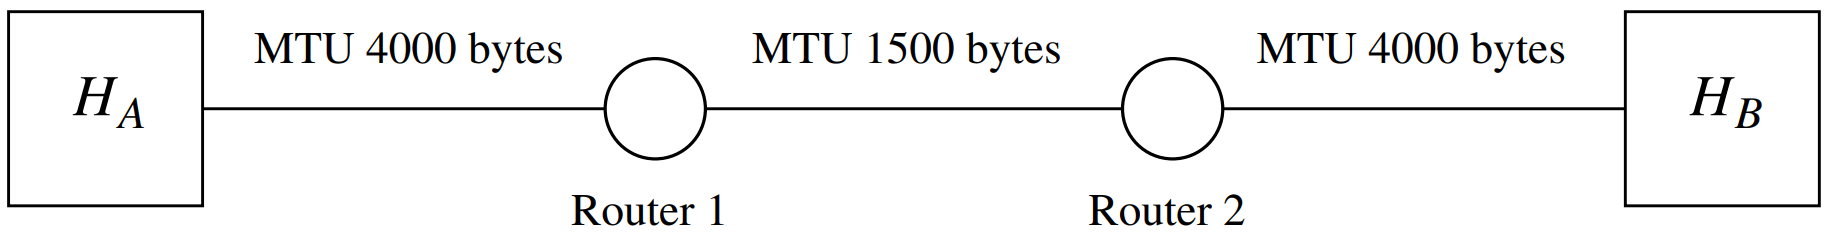
\includegraphics[width=\textwidth]{router_diagram}
\end{center}

$H_A$ chooses a TCP segment size of 3000 bytes of data (TCP and IP headers
are each 20 bytes in size).

\begin{enumerate}
[label=(\roman*)]

\item Describe the way in which fragmentation takes place as $H_A$ sends data
to $H_B$. Include the arithmetic used to calculate fragment sizes. Explain
the saving that may be made by $H_A$ choosing an optimal TCP segment
size when sending 60KBytes of data.

I assume the header of the IP packet is \textit{not} included in the TCP
segment size, but the TCP header is included in the size of the TCP segment.
So the IP packet sent from $H_A$ will be $3020$ bytes large.

In IPv4, packets are fragmented at intermediate nodes if the MTU for the
next link is smaller than the packet size. When the packet arrives at router
1, it is larger than the MTU for the next link on the route. So the router
will fragment the packet. Each will have a fragment offset. In this case,
the packet will be fragmented into three smaller packets: the first two
packets will contain the TCP header, an IP header and have 1460 bytes of
payload. The final packet will contain the TCP header, an IP header and 1060
bytes of payload.

In IPv4, reconstruction is only done at the destination. IPv4 packets use a
fragment offset rather than a fragment number since packets can be
fragmented at multiple nodes. Note that a layering violation is required to
ensure that each packet contains enough information to reconstruct it at
the destination.

The downside of en-route fragmentation is that if even one of the fragments
is lost, then the TCP segment cannot be delivered. Hence the sender will
have to retransmit the entire TCP segment. This wastes network bandwidth and
increases latency.

The optimal segment size is the MTU for the link with the least capacity.
So the optimal segment size is 1480 bytes (such that with the IP header,
the IP packet will be the MTU).

\item Briefly explain how the situation described in part (i) would be
handled if Internet Protocol version 6 (IPv6) were used.

IPv6 does not do any en-route fragmentation. If the case above was using
IPv6, the segments would be dropped at Router 1 and an ICMP error message
would be sent to $H_A$.

\end{enumerate}

\item The formulae below are used in TCP implementations to compute a
value for the retransmission time-out ($R$). $R$ is an estimate of the
round-trip time, $M$ is the most recently measured round-trip measurement,
$\alpha = 0.875$ and $h = 0.25$.
\begin{align*}
D &\leftarrow D + h(|M - R| - D) \\
R &\leftarrow \alpha R + (a - \alpha)M \\
\mathcal{R} &= R + 4D
\end{align*}
\begin{enumerate}[label=(\roman*)]

\item How is $M$ measured?

Read the clock when the message is sent, and read it when the response
arrives from $H_B$. However, if we have to request a retransmission then we
should not measure $M$ -- since it's impossible to tell whether the response
was for the original message we sent or for the retransmission.

\item Explain the principles behind the design of these formulae and the
values $h$, $\alpha$ and $D$.

This is the Jacobson/Karels algorithm.

$D$ is the deviation of the round-trip time. $h$ is a constant used in the
exponential weighted average of $D$ and $\alpha$ is a constant used in the
exponential weighted average of the round-trip time and $\mathcal R$ is the
timeout.

We assume that the mean and variance of the round trip time are not known
and are variable. However, we can estimate both of them using an
exponential-weighted average. Whatever distribution the latency of
correctly delivered packets is drawn from, the probability of a packet
being delayed by more than 4 deviations is very small. So if the latency
reaches this, we resent the request. This takes into account both the
latency and the round trip time and so generalises well to many different
types of network under many different loads.

Large timeouts occur when either the mean of the $\mathop{RTT}$ is very
large, or the variance is very large. Either of these imply that a large
delay would not be unlikely. Small timeouts occur if and only if both the
mean $\mathop{RTT}$ and the deviation is very low.

We use $\alpha = 0.875$ because this is $\frac{7}{8}$. It can be easily
calculated by bit-shifts. Similar reasoning for why $h = 0.25$ -- it can be
calculated in a single bit-shift. Since all of these calculations are
carried out many times, we want the arithmetic to be as simple as possible.

Note that the expectation of $R$ is given by $\frac{a -
\alpha}{1 - \alpha}\mathop{RTT}$. Therefore, $a$ must be equal to 1 to
ensure that the expectation of the estimate for the round-trip time is the
round trip time.

\end{enumerate}

\end{enumerate}

\end{examquestion}

\end{document}
